\documentclass[compress,11pt]{beamer}
%\includeonly{pendel}
\usetheme{Ilmenau}
%\usetheme{fau-4-3}
%\usecolortheme{beaver}
\beamertemplatenavigationsymbolsempty
\usepackage[ngerman]{babel}
\usepackage{marvosym}
\usepackage{multimedia}
\usepackage[utf8]{inputenc}
\usepackage{amsmath}
\usepackage{amsfonts}
\usepackage{amssymb}
\usepackage{graphicx}
\usepackage{esvect}
%\author{}
\title{EP Gruppe 8}
%\setbeamercovered{transparent}
%\setbeamertemplate{navigation symbols}{}
%\logo{}
%\institute{}
%\date{}
%\subject{}
\usepackage{verbatim}
\begin{document}

\frame[c]{\titlepage}
\begin{frame}
\tableofcontents
\end{frame}

\section{Aufgabe 1}
\subsection{a)}
\begin{frame}{Innenwiderstand}
\begin{block}{Shuntwiderstand im DMM}
%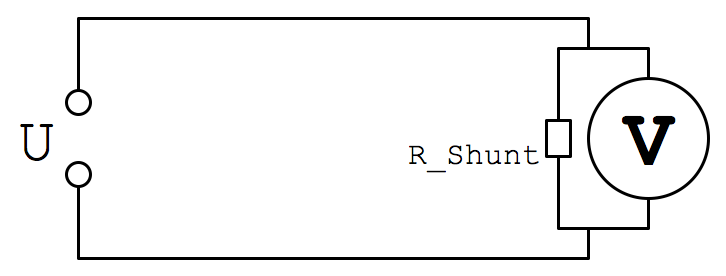
\includegraphics[width=\textwidth]{images/1a.png} %Schaltbild
\end{block}
\end{frame}
\section{Aufgabe 3}
\begin{frame}
\begin{block}{Gegebene Schaltung}
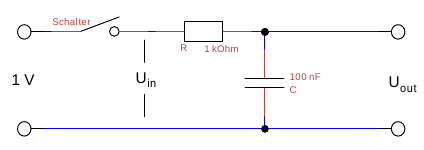
\includegraphics[width=\textwidth]{../daten/Messdaten/plots/schalt_tief2}
\end{block}
\end{frame}
\begin{frame}
Gemessene3 Sprungreaktion:\\
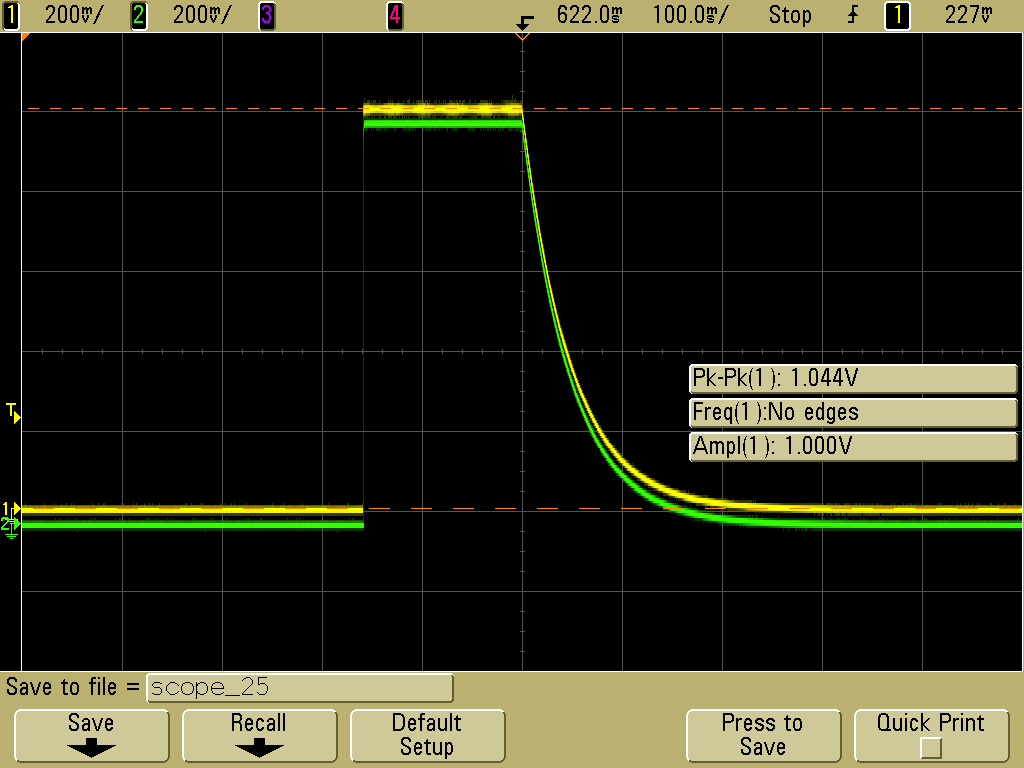
\includegraphics[width=\textwidth]{../daten/scope_25}
\end{frame}
\begin{frame}
Gesucht: Zeitkonstante $\tau = R \cdot C$\\
Sprungreaktion ist in diesem Fall der Entladevorgang des Kondensators, gegeben durch:
\begin{equation}
U(t) = U_0 * \exp(-\frac{t}{\tau}),  \tau = \frac{1}{R\cdot C}
\end{equation}
\end{frame}
\begin{frame}
Strategie: Setze $t=\tau$ $\Rightarrow  U(\tau) = U_0 \cdot \exp(-1)$\\
und suche den Wert $\frac{U(t)}{U_0} = \frac{1}{e}$ in der Messtabelle:
\begin{equation}
t \approx 0.045 s
\end{equation}
Errechneter Wert:
\begin{equation}
\tau = R \cdot C = 10^{-7} \cdot 10^{3} = 10^{-4}
\end{equation}
\end{frame}
\section{Aufgabe 4}
\begin{frame}
\begin{block}{Das fehlende Bauelement ist eine Drossel}
\centering
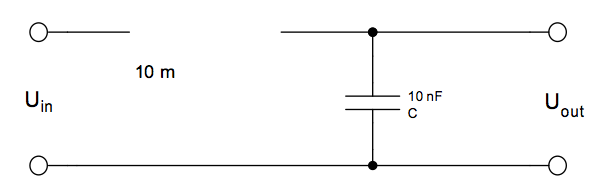
\includegraphics[width=\textwidth]{../daten/Messdaten/plots/schalt_4spule.png}
\end{block}
\end{frame}

\begin{frame}
\begin{block}{Messung mit Spule allein}
\centering
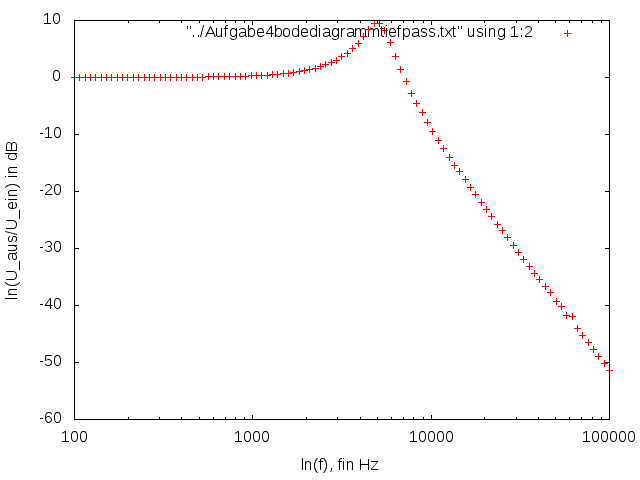
\includegraphics[width=.85\textwidth]{../daten/Messdaten/plots/Aufgabe4Bodediagramm_tief_gain}
\end{block}
\end{frame}

\begin{frame}
\begin{block}{Zweite Messung mit Widerstand in Reihe zur Spule}
\centering
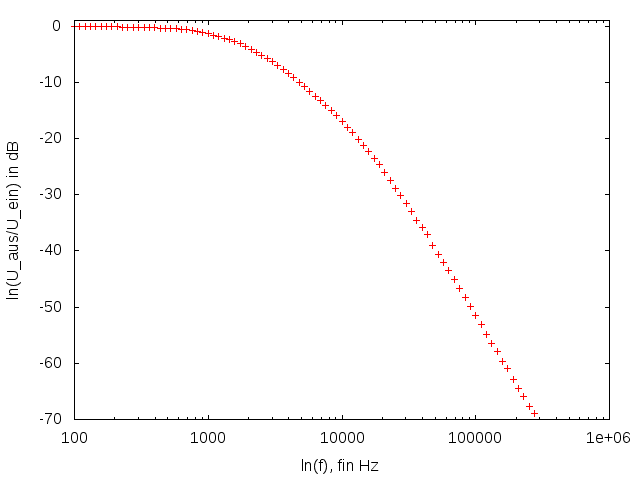
\includegraphics[width=0.85\textwidth]{../daten/Messdaten/plots/Aufgabe4Bodediagramm_tief_R_gain}
\end{block}
\end{frame}
\end{document}
